% Options for packages loaded elsewhere
\PassOptionsToPackage{unicode}{hyperref}
\PassOptionsToPackage{hyphens}{url}
\PassOptionsToPackage{dvipsnames,svgnames,x11names}{xcolor}
%
\documentclass[
  letterpaper,
  DIV=11,
  numbers=noendperiod]{scrartcl}

\usepackage{amsmath,amssymb}
\usepackage{iftex}
\ifPDFTeX
  \usepackage[T1]{fontenc}
  \usepackage[utf8]{inputenc}
  \usepackage{textcomp} % provide euro and other symbols
\else % if luatex or xetex
  \usepackage{unicode-math}
  \defaultfontfeatures{Scale=MatchLowercase}
  \defaultfontfeatures[\rmfamily]{Ligatures=TeX,Scale=1}
\fi
\usepackage{lmodern}
\ifPDFTeX\else  
    % xetex/luatex font selection
\fi
% Use upquote if available, for straight quotes in verbatim environments
\IfFileExists{upquote.sty}{\usepackage{upquote}}{}
\IfFileExists{microtype.sty}{% use microtype if available
  \usepackage[]{microtype}
  \UseMicrotypeSet[protrusion]{basicmath} % disable protrusion for tt fonts
}{}
\makeatletter
\@ifundefined{KOMAClassName}{% if non-KOMA class
  \IfFileExists{parskip.sty}{%
    \usepackage{parskip}
  }{% else
    \setlength{\parindent}{0pt}
    \setlength{\parskip}{6pt plus 2pt minus 1pt}}
}{% if KOMA class
  \KOMAoptions{parskip=half}}
\makeatother
\usepackage{xcolor}
\setlength{\emergencystretch}{3em} % prevent overfull lines
\setcounter{secnumdepth}{-\maxdimen} % remove section numbering
% Make \paragraph and \subparagraph free-standing
\ifx\paragraph\undefined\else
  \let\oldparagraph\paragraph
  \renewcommand{\paragraph}[1]{\oldparagraph{#1}\mbox{}}
\fi
\ifx\subparagraph\undefined\else
  \let\oldsubparagraph\subparagraph
  \renewcommand{\subparagraph}[1]{\oldsubparagraph{#1}\mbox{}}
\fi

\usepackage{color}
\usepackage{fancyvrb}
\newcommand{\VerbBar}{|}
\newcommand{\VERB}{\Verb[commandchars=\\\{\}]}
\DefineVerbatimEnvironment{Highlighting}{Verbatim}{commandchars=\\\{\}}
% Add ',fontsize=\small' for more characters per line
\usepackage{framed}
\definecolor{shadecolor}{RGB}{241,243,245}
\newenvironment{Shaded}{\begin{snugshade}}{\end{snugshade}}
\newcommand{\AlertTok}[1]{\textcolor[rgb]{0.68,0.00,0.00}{#1}}
\newcommand{\AnnotationTok}[1]{\textcolor[rgb]{0.37,0.37,0.37}{#1}}
\newcommand{\AttributeTok}[1]{\textcolor[rgb]{0.40,0.45,0.13}{#1}}
\newcommand{\BaseNTok}[1]{\textcolor[rgb]{0.68,0.00,0.00}{#1}}
\newcommand{\BuiltInTok}[1]{\textcolor[rgb]{0.00,0.23,0.31}{#1}}
\newcommand{\CharTok}[1]{\textcolor[rgb]{0.13,0.47,0.30}{#1}}
\newcommand{\CommentTok}[1]{\textcolor[rgb]{0.37,0.37,0.37}{#1}}
\newcommand{\CommentVarTok}[1]{\textcolor[rgb]{0.37,0.37,0.37}{\textit{#1}}}
\newcommand{\ConstantTok}[1]{\textcolor[rgb]{0.56,0.35,0.01}{#1}}
\newcommand{\ControlFlowTok}[1]{\textcolor[rgb]{0.00,0.23,0.31}{#1}}
\newcommand{\DataTypeTok}[1]{\textcolor[rgb]{0.68,0.00,0.00}{#1}}
\newcommand{\DecValTok}[1]{\textcolor[rgb]{0.68,0.00,0.00}{#1}}
\newcommand{\DocumentationTok}[1]{\textcolor[rgb]{0.37,0.37,0.37}{\textit{#1}}}
\newcommand{\ErrorTok}[1]{\textcolor[rgb]{0.68,0.00,0.00}{#1}}
\newcommand{\ExtensionTok}[1]{\textcolor[rgb]{0.00,0.23,0.31}{#1}}
\newcommand{\FloatTok}[1]{\textcolor[rgb]{0.68,0.00,0.00}{#1}}
\newcommand{\FunctionTok}[1]{\textcolor[rgb]{0.28,0.35,0.67}{#1}}
\newcommand{\ImportTok}[1]{\textcolor[rgb]{0.00,0.46,0.62}{#1}}
\newcommand{\InformationTok}[1]{\textcolor[rgb]{0.37,0.37,0.37}{#1}}
\newcommand{\KeywordTok}[1]{\textcolor[rgb]{0.00,0.23,0.31}{#1}}
\newcommand{\NormalTok}[1]{\textcolor[rgb]{0.00,0.23,0.31}{#1}}
\newcommand{\OperatorTok}[1]{\textcolor[rgb]{0.37,0.37,0.37}{#1}}
\newcommand{\OtherTok}[1]{\textcolor[rgb]{0.00,0.23,0.31}{#1}}
\newcommand{\PreprocessorTok}[1]{\textcolor[rgb]{0.68,0.00,0.00}{#1}}
\newcommand{\RegionMarkerTok}[1]{\textcolor[rgb]{0.00,0.23,0.31}{#1}}
\newcommand{\SpecialCharTok}[1]{\textcolor[rgb]{0.37,0.37,0.37}{#1}}
\newcommand{\SpecialStringTok}[1]{\textcolor[rgb]{0.13,0.47,0.30}{#1}}
\newcommand{\StringTok}[1]{\textcolor[rgb]{0.13,0.47,0.30}{#1}}
\newcommand{\VariableTok}[1]{\textcolor[rgb]{0.07,0.07,0.07}{#1}}
\newcommand{\VerbatimStringTok}[1]{\textcolor[rgb]{0.13,0.47,0.30}{#1}}
\newcommand{\WarningTok}[1]{\textcolor[rgb]{0.37,0.37,0.37}{\textit{#1}}}

\providecommand{\tightlist}{%
  \setlength{\itemsep}{0pt}\setlength{\parskip}{0pt}}\usepackage{longtable,booktabs,array}
\usepackage{calc} % for calculating minipage widths
% Correct order of tables after \paragraph or \subparagraph
\usepackage{etoolbox}
\makeatletter
\patchcmd\longtable{\par}{\if@noskipsec\mbox{}\fi\par}{}{}
\makeatother
% Allow footnotes in longtable head/foot
\IfFileExists{footnotehyper.sty}{\usepackage{footnotehyper}}{\usepackage{footnote}}
\makesavenoteenv{longtable}
\usepackage{graphicx}
\makeatletter
\def\maxwidth{\ifdim\Gin@nat@width>\linewidth\linewidth\else\Gin@nat@width\fi}
\def\maxheight{\ifdim\Gin@nat@height>\textheight\textheight\else\Gin@nat@height\fi}
\makeatother
% Scale images if necessary, so that they will not overflow the page
% margins by default, and it is still possible to overwrite the defaults
% using explicit options in \includegraphics[width, height, ...]{}
\setkeys{Gin}{width=\maxwidth,height=\maxheight,keepaspectratio}
% Set default figure placement to htbp
\makeatletter
\def\fps@figure{htbp}
\makeatother

\usepackage{fontspec}
\usepackage{multirow}
\usepackage{multicol}
\usepackage{colortbl}
\usepackage{hhline}
\newlength\Oldarrayrulewidth
\newlength\Oldtabcolsep
\usepackage{longtable}
\usepackage{array}
\usepackage{hyperref}
\usepackage{float}
\usepackage{wrapfig}
\usepackage{tabularray}
\usepackage[normalem]{ulem}
\usepackage{graphicx}
\UseTblrLibrary{booktabs}
\UseTblrLibrary{siunitx}
\NewTableCommand{\tinytableDefineColor}[3]{\definecolor{#1}{#2}{#3}}
\newcommand{\tinytableTabularrayUnderline}[1]{\underline{#1}}
\newcommand{\tinytableTabularrayStrikeout}[1]{\sout{#1}}
\KOMAoption{captions}{tableheading}
\makeatletter
\makeatother
\makeatletter
\makeatother
\makeatletter
\@ifpackageloaded{caption}{}{\usepackage{caption}}
\AtBeginDocument{%
\ifdefined\contentsname
  \renewcommand*\contentsname{Table of contents}
\else
  \newcommand\contentsname{Table of contents}
\fi
\ifdefined\listfigurename
  \renewcommand*\listfigurename{List of Figures}
\else
  \newcommand\listfigurename{List of Figures}
\fi
\ifdefined\listtablename
  \renewcommand*\listtablename{List of Tables}
\else
  \newcommand\listtablename{List of Tables}
\fi
\ifdefined\figurename
  \renewcommand*\figurename{Figure}
\else
  \newcommand\figurename{Figure}
\fi
\ifdefined\tablename
  \renewcommand*\tablename{Table}
\else
  \newcommand\tablename{Table}
\fi
}
\@ifpackageloaded{float}{}{\usepackage{float}}
\floatstyle{ruled}
\@ifundefined{c@chapter}{\newfloat{codelisting}{h}{lop}}{\newfloat{codelisting}{h}{lop}[chapter]}
\floatname{codelisting}{Listing}
\newcommand*\listoflistings{\listof{codelisting}{List of Listings}}
\makeatother
\makeatletter
\@ifpackageloaded{caption}{}{\usepackage{caption}}
\@ifpackageloaded{subcaption}{}{\usepackage{subcaption}}
\makeatother
\makeatletter
\@ifpackageloaded{tcolorbox}{}{\usepackage[skins,breakable]{tcolorbox}}
\makeatother
\makeatletter
\@ifundefined{shadecolor}{\definecolor{shadecolor}{rgb}{.97, .97, .97}}
\makeatother
\makeatletter
\makeatother
\makeatletter
\makeatother
\ifLuaTeX
  \usepackage{selnolig}  % disable illegal ligatures
\fi
\IfFileExists{bookmark.sty}{\usepackage{bookmark}}{\usepackage{hyperref}}
\IfFileExists{xurl.sty}{\usepackage{xurl}}{} % add URL line breaks if available
\urlstyle{same} % disable monospaced font for URLs
\hypersetup{
  pdftitle={Homework 3},
  pdfauthor={Odile Gabbiani},
  colorlinks=true,
  linkcolor={blue},
  filecolor={Maroon},
  citecolor={Blue},
  urlcolor={Blue},
  pdfcreator={LaTeX via pandoc}}

\title{Homework 3}
\author{Odile Gabbiani}
\date{}

\begin{document}
\maketitle
\ifdefined\Shaded\renewenvironment{Shaded}{\begin{tcolorbox}[breakable, sharp corners, interior hidden, borderline west={3pt}{0pt}{shadecolor}, frame hidden, enhanced, boxrule=0pt]}{\end{tcolorbox}}\fi

\renewcommand*\contentsname{Table of contents}
{
\hypersetup{linkcolor=}
\setcounter{tocdepth}{3}
\tableofcontents
}
\hypertarget{quarto}{%
\subsection{Quarto}\label{quarto}}

Quarto enables you to weave together content and executable code into a
finished document. To learn more about Quarto see
\url{https://quarto.org}.

\hypertarget{running-code}{%
\subsection{Running Code}\label{running-code}}

When you click the \textbf{Render} button a document will be generated
that includes both content and the output of embedded code. You can
embed code like this:

\begin{Shaded}
\begin{Highlighting}[]
\FunctionTok{library}\NormalTok{(tidyverse)}
\FunctionTok{library}\NormalTok{(readxl)}
\FunctionTok{library}\NormalTok{(here)}
\FunctionTok{library}\NormalTok{(janitor)}
\FunctionTok{library}\NormalTok{(GGally)}
\FunctionTok{library}\NormalTok{(MuMIn)}
\FunctionTok{library}\NormalTok{(ggeffects)}
\FunctionTok{library}\NormalTok{(gtsummary)}
\FunctionTok{library}\NormalTok{(flextable)}
\FunctionTok{library}\NormalTok{(modelsummary)}

\NormalTok{drought\_exp }\OtherTok{\textless{}{-}} \FunctionTok{read\_xlsx}\NormalTok{(}\AttributeTok{path =} \FunctionTok{here}\NormalTok{(}\StringTok{"data"}\NormalTok{, }
                                     \StringTok{"Valliere\_etal\_EcoApps\_Data.xlsx"}\NormalTok{),}
                         \AttributeTok{sheet =} \StringTok{"First Harvest"}\NormalTok{)}

\CommentTok{\# quick look at data }
\FunctionTok{str}\NormalTok{(drought\_exp)}
\end{Highlighting}
\end{Shaded}

\begin{verbatim}
tibble [70 x 13] (S3: tbl_df/tbl/data.frame)
 $ Species            : chr [1:70] "ENCCAL" "ENCCAL" "ENCCAL" "ENCCAL" ...
 $ Water              : chr [1:70] "WW" "WW" "WW" "WW" ...
 $ Rep #              : num [1:70] 1 2 3 4 5 1 2 3 4 5 ...
 $ Height (cm)        : num [1:70] 5.8 4.9 8.4 6.5 7.1 3.2 4.4 4.2 4.5 3.9 ...
 $ Leaf #             : num [1:70] 11 8 11 12 10 7 7 10 8 6 ...
 $ Leaf dry weight (g): num [1:70] 0.0294 0.0185 0.0177 0.0178 0.0164 0.017 0.0193 0.0153 0.0159 0.0133 ...
 $ Leaf area (cm2)    : num [1:70] 5.01 3.98 3.69 3.84 3.63 3.06 3.1 2.94 2.73 2.61 ...
 $ SLA                : num [1:70] 170 215 209 216 222 ...
 $ Total LA           : num [1:70] 55.1 31.8 40.6 46.1 36.3 ...
 $ Shoot (g)          : num [1:70] 0.253 0.164 0.241 0.213 0.232 ...
 $ Root (g)           : num [1:70] 0.202 0.165 0.209 0.146 0.12 ...
 $ Total (g)          : num [1:70] 0.455 0.329 0.45 0.359 0.352 ...
 $ R:S                : num [1:70] 0.8 1 0.9 0.7 0.5 0.8 1.2 3.1 0.9 1.2 ...
\end{verbatim}

\begin{Shaded}
\begin{Highlighting}[]
\FunctionTok{class}\NormalTok{(drought\_exp)}
\end{Highlighting}
\end{Shaded}

\begin{verbatim}
[1] "tbl_df"     "tbl"        "data.frame"
\end{verbatim}

You can add options to executable code like this

\begin{Shaded}
\begin{Highlighting}[]
\NormalTok{drought\_exp\_clean }\OtherTok{\textless{}{-}}\NormalTok{ drought\_exp }\SpecialCharTok{\%\textgreater{}\%} 
  \FunctionTok{clean\_names}\NormalTok{() }\SpecialCharTok{\%\textgreater{}\%} \CommentTok{\# nicer column names}
  \FunctionTok{mutate}\NormalTok{(}\AttributeTok{species\_name =} \FunctionTok{case\_when}\NormalTok{( }\CommentTok{\# adding column with species scientific names}
\NormalTok{    species }\SpecialCharTok{==} \StringTok{"ENCCAL"} \SpecialCharTok{\textasciitilde{}} \StringTok{"Encelia californica"}\NormalTok{, }\CommentTok{\# bush sunflower}
\NormalTok{    species }\SpecialCharTok{==} \StringTok{"ESCCAL"} \SpecialCharTok{\textasciitilde{}} \StringTok{"Eschscholzia californica"}\NormalTok{, }\CommentTok{\# California poppy}
\NormalTok{    species }\SpecialCharTok{==} \StringTok{"PENCEN"} \SpecialCharTok{\textasciitilde{}} \StringTok{"Penstemon centranthifolius"}\NormalTok{, }\CommentTok{\# Scarlet bugler}
\NormalTok{    species }\SpecialCharTok{==} \StringTok{"GRICAM"} \SpecialCharTok{\textasciitilde{}} \StringTok{"Grindelia camporum"}\NormalTok{, }\CommentTok{\# great valley gumweed}
\NormalTok{    species }\SpecialCharTok{==} \StringTok{"SALLEU"} \SpecialCharTok{\textasciitilde{}} \StringTok{"Salvia leucophylla"}\NormalTok{, }\CommentTok{\# Purple sage}
\NormalTok{    species }\SpecialCharTok{==} \StringTok{"STIPUL"} \SpecialCharTok{\textasciitilde{}} \StringTok{"Nasella pulchra"}\NormalTok{, }\CommentTok{\# Purple needlegrass}
\NormalTok{    species }\SpecialCharTok{==} \StringTok{"LOTSCO"} \SpecialCharTok{\textasciitilde{}} \StringTok{"Acmispon glaber"} \CommentTok{\# deerweed}
\NormalTok{  )) }\SpecialCharTok{\%\textgreater{}\%} 
  \FunctionTok{relocate}\NormalTok{(species\_name, }\AttributeTok{.after =}\NormalTok{ species) }\SpecialCharTok{\%\textgreater{}\%} \CommentTok{\# moving species\_name column after species}
  \FunctionTok{mutate}\NormalTok{(}\AttributeTok{water\_treatment =} \FunctionTok{case\_when}\NormalTok{( }\CommentTok{\# adding column with full treatment names}
\NormalTok{    water }\SpecialCharTok{==} \StringTok{"WW"} \SpecialCharTok{\textasciitilde{}} \StringTok{"Well watered"}\NormalTok{,}
\NormalTok{    water }\SpecialCharTok{==} \StringTok{"DS"} \SpecialCharTok{\textasciitilde{}} \StringTok{"Drought stressed"}
\NormalTok{  )) }\SpecialCharTok{\%\textgreater{}\%} 
  \FunctionTok{relocate}\NormalTok{(water\_treatment, }\AttributeTok{.after =}\NormalTok{ water) }\CommentTok{\# moving water\_treatment column after water}
\end{Highlighting}
\end{Shaded}

\begin{Shaded}
\begin{Highlighting}[]
\FunctionTok{ggpairs}\NormalTok{(drought\_exp\_clean, }\CommentTok{\# data frame}
        \AttributeTok{columns =} \FunctionTok{c}\NormalTok{(}\StringTok{"leaf\_dry\_weight\_g"}\NormalTok{, }\CommentTok{\# columns to visualize}
                    \StringTok{"sla"}\NormalTok{, }
                    \StringTok{"shoot\_g"}\NormalTok{, }
                    \StringTok{"root\_g"}\NormalTok{, }
                    \StringTok{"total\_g"}\NormalTok{), }
        \AttributeTok{upper =} \FunctionTok{list}\NormalTok{(}\AttributeTok{method =} \StringTok{"pearson"}\NormalTok{)) }\SpecialCharTok{+} \CommentTok{\# calculating Pearson correlation coefficient}
  \FunctionTok{theme\_bw}\NormalTok{() }\SpecialCharTok{+} \CommentTok{\# cleaner theme}
  \FunctionTok{theme}\NormalTok{(}\AttributeTok{panel.grid =} \FunctionTok{element\_blank}\NormalTok{()) }\CommentTok{\# getting rid of gridlines}
\end{Highlighting}
\end{Shaded}

\begin{figure}[H]

{\centering 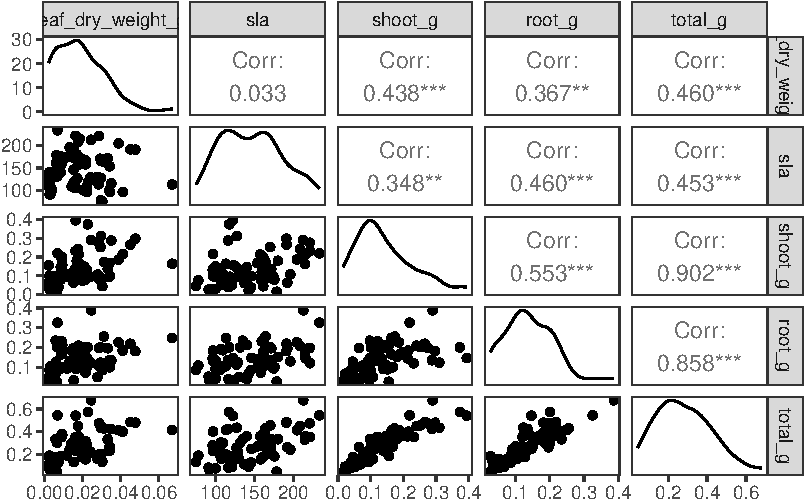
\includegraphics{Odile_Gabbiani_homework-03_files/figure-pdf/unnamed-chunk-3-1.pdf}

}

\end{figure}

\begin{Shaded}
\begin{Highlighting}[]
\FunctionTok{ggplot}\NormalTok{(}\AttributeTok{data =}\NormalTok{ drought\_exp\_clean, }\CommentTok{\# data frame}
       \FunctionTok{aes}\NormalTok{(}\AttributeTok{x =} \FunctionTok{reorder}\NormalTok{(species\_name, }\CommentTok{\# reordering x{-}axis}
                       \SpecialCharTok{{-}}\NormalTok{total\_g, }\CommentTok{\# in reverse order of mean total mass}
                       \AttributeTok{fun =}\NormalTok{ mean), }\CommentTok{\# calculating mean to reorder}
           \AttributeTok{y =}\NormalTok{ total\_g)) }\SpecialCharTok{+} \CommentTok{\# y{-}axis}
  \FunctionTok{geom\_jitter}\NormalTok{(}\AttributeTok{width =} \FloatTok{0.1}\NormalTok{, }\CommentTok{\# narrow jitter}
              \AttributeTok{height =} \DecValTok{0}\NormalTok{) }\CommentTok{\# not jittering points up and down}
\end{Highlighting}
\end{Shaded}

\begin{figure}[H]

{\centering 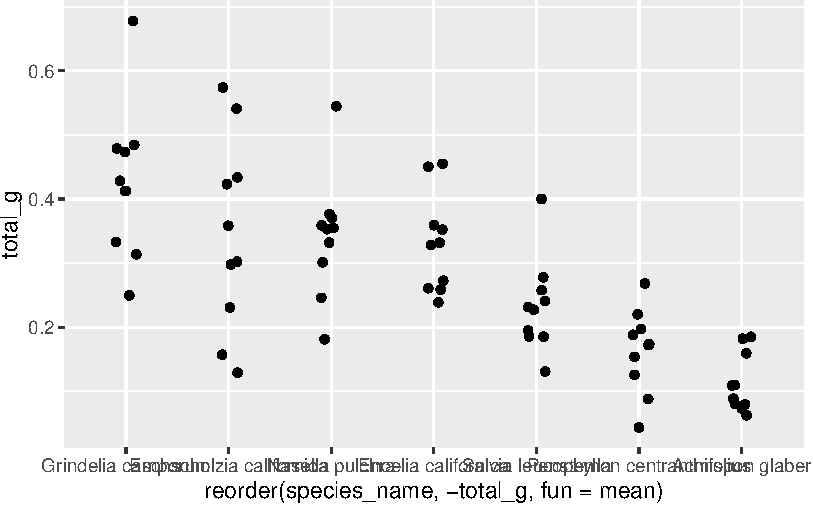
\includegraphics{Odile_Gabbiani_homework-03_files/figure-pdf/unnamed-chunk-4-1.pdf}

}

\end{figure}

\begin{Shaded}
\begin{Highlighting}[]
\FunctionTok{ggplot}\NormalTok{(}\AttributeTok{data =}\NormalTok{ drought\_exp\_clean, }\CommentTok{\# data frame}
       \FunctionTok{aes}\NormalTok{(}\AttributeTok{x =}\NormalTok{ water\_treatment, }\CommentTok{\# x{-}axis}
           \AttributeTok{y =}\NormalTok{ total\_g)) }\SpecialCharTok{+} \CommentTok{\# y{-}axis}
  \FunctionTok{geom\_jitter}\NormalTok{(}\AttributeTok{width =} \FloatTok{0.1}\NormalTok{, }\CommentTok{\# narrow jitter}
              \AttributeTok{height =} \DecValTok{0}\NormalTok{) }\CommentTok{\# not jittering points up and down}
\end{Highlighting}
\end{Shaded}

\begin{figure}[H]

{\centering 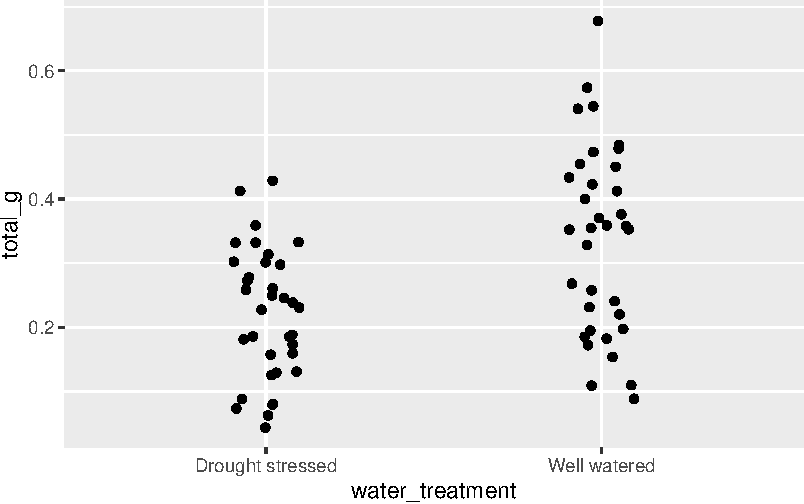
\includegraphics{Odile_Gabbiani_homework-03_files/figure-pdf/unnamed-chunk-5-1.pdf}

}

\end{figure}

\begin{Shaded}
\begin{Highlighting}[]
\FunctionTok{ggplot}\NormalTok{(}\AttributeTok{data =}\NormalTok{ drought\_exp\_clean, }\CommentTok{\# data frame}
       \FunctionTok{aes}\NormalTok{(}\AttributeTok{x =}\NormalTok{ sla, }\CommentTok{\# x{-}axis}
           \AttributeTok{y =}\NormalTok{ total\_g)) }\SpecialCharTok{+} \CommentTok{\# y{-}axis}
  \FunctionTok{geom\_point}\NormalTok{() }\CommentTok{\# scatterplot}
\end{Highlighting}
\end{Shaded}

\begin{figure}[H]

{\centering 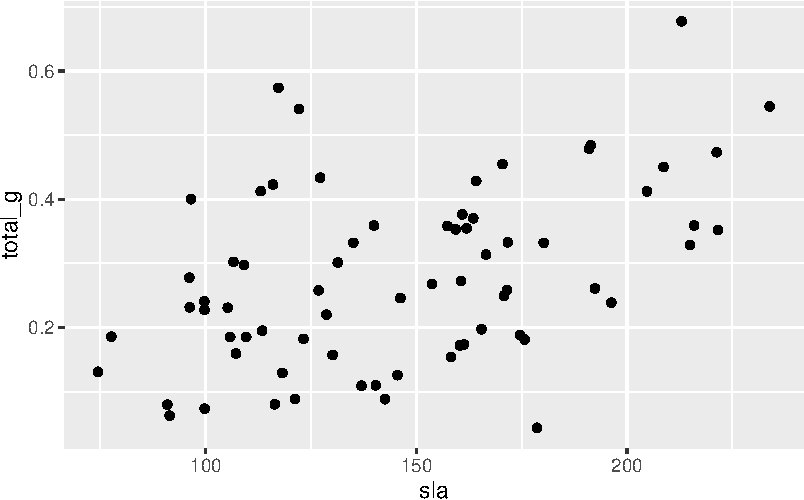
\includegraphics{Odile_Gabbiani_homework-03_files/figure-pdf/unnamed-chunk-6-1.pdf}

}

\end{figure}

\begin{Shaded}
\begin{Highlighting}[]
\NormalTok{model0 }\OtherTok{\textless{}{-}} \FunctionTok{lm}\NormalTok{(total\_g }\SpecialCharTok{\textasciitilde{}} \DecValTok{1}\NormalTok{, }\CommentTok{\# formula}
             \AttributeTok{data =}\NormalTok{ drought\_exp\_clean) }\CommentTok{\# data frame}
\end{Highlighting}
\end{Shaded}

\begin{Shaded}
\begin{Highlighting}[]
\NormalTok{model1 }\OtherTok{\textless{}{-}} \FunctionTok{lm}\NormalTok{(total\_g }\SpecialCharTok{\textasciitilde{}}\NormalTok{ sla }\SpecialCharTok{+}\NormalTok{ water\_treatment }\SpecialCharTok{+}\NormalTok{ species\_name,}
             \AttributeTok{data =}\NormalTok{ drought\_exp\_clean)}

\FunctionTok{par}\NormalTok{(}\AttributeTok{mfrow =} \FunctionTok{c}\NormalTok{(}\DecValTok{2}\NormalTok{, }\DecValTok{2}\NormalTok{))}
\FunctionTok{plot}\NormalTok{(model1)}
\end{Highlighting}
\end{Shaded}

\begin{figure}[H]

{\centering 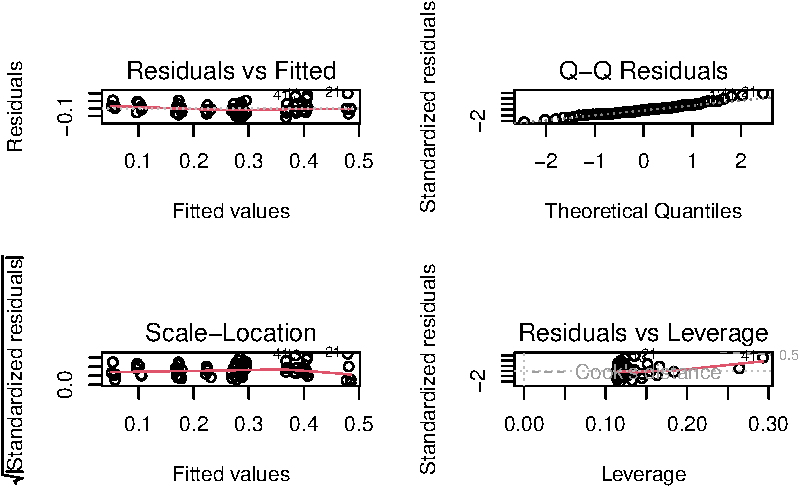
\includegraphics{Odile_Gabbiani_homework-03_files/figure-pdf/unnamed-chunk-8-1.pdf}

}

\end{figure}

\begin{Shaded}
\begin{Highlighting}[]
\CommentTok{\# you might get a warning when you run this code {-} that is ok!}
\end{Highlighting}
\end{Shaded}

\begin{Shaded}
\begin{Highlighting}[]
\NormalTok{model2 }\OtherTok{\textless{}{-}} \FunctionTok{lm}\NormalTok{(total\_g }\SpecialCharTok{\textasciitilde{}}\NormalTok{ sla }\SpecialCharTok{+}\NormalTok{ water\_treatment,}
             \AttributeTok{data =}\NormalTok{ drought\_exp\_clean)}

\FunctionTok{plot}\NormalTok{(model2)}
\end{Highlighting}
\end{Shaded}

\begin{figure}[H]

{\centering 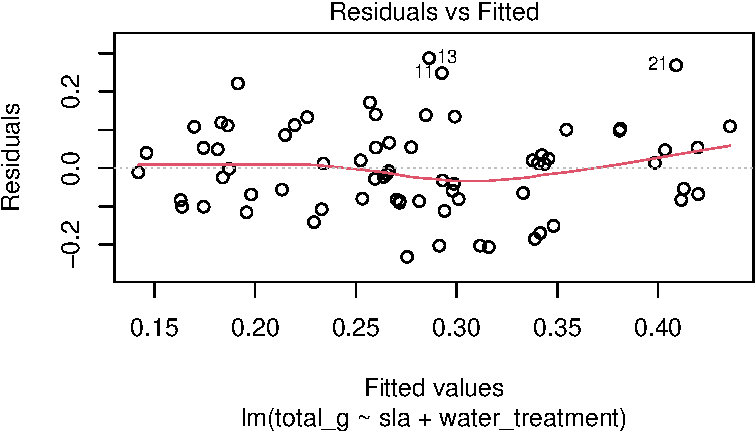
\includegraphics{Odile_Gabbiani_homework-03_files/figure-pdf/unnamed-chunk-9-1.pdf}

}

\end{figure}

\begin{figure}[H]

{\centering 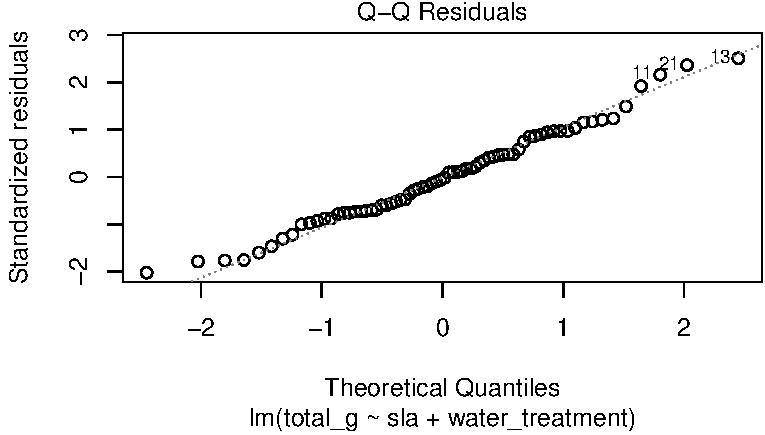
\includegraphics{Odile_Gabbiani_homework-03_files/figure-pdf/unnamed-chunk-9-2.pdf}

}

\end{figure}

\begin{figure}[H]

{\centering 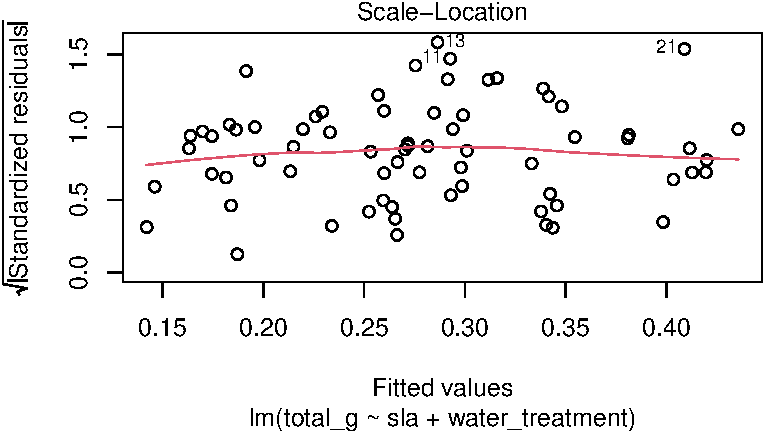
\includegraphics{Odile_Gabbiani_homework-03_files/figure-pdf/unnamed-chunk-9-3.pdf}

}

\end{figure}

\begin{figure}[H]

{\centering 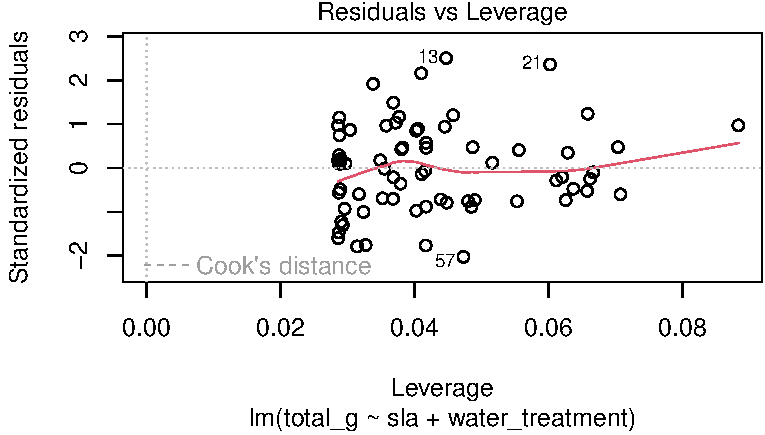
\includegraphics{Odile_Gabbiani_homework-03_files/figure-pdf/unnamed-chunk-9-4.pdf}

}

\end{figure}

\begin{Shaded}
\begin{Highlighting}[]
\NormalTok{model3 }\OtherTok{\textless{}{-}} \FunctionTok{lm}\NormalTok{(total\_g }\SpecialCharTok{\textasciitilde{}}\NormalTok{ sla }\SpecialCharTok{+}\NormalTok{ species\_name,}
             \AttributeTok{data =}\NormalTok{ drought\_exp\_clean)}

\FunctionTok{plot}\NormalTok{(model3)}
\end{Highlighting}
\end{Shaded}

\begin{figure}[H]

{\centering 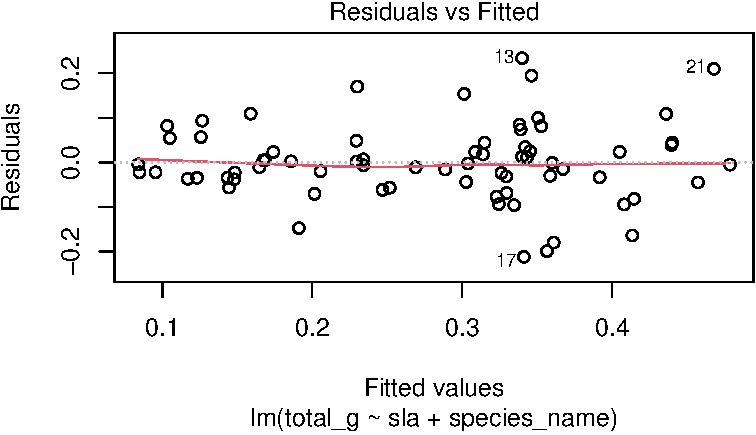
\includegraphics{Odile_Gabbiani_homework-03_files/figure-pdf/unnamed-chunk-10-1.pdf}

}

\end{figure}

\begin{figure}[H]

{\centering 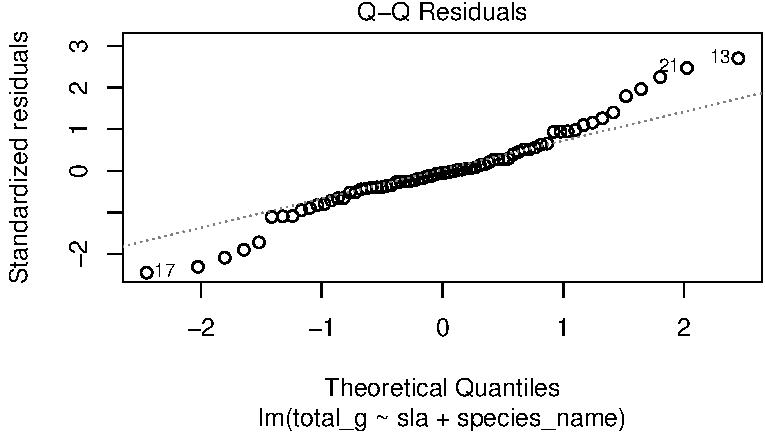
\includegraphics{Odile_Gabbiani_homework-03_files/figure-pdf/unnamed-chunk-10-2.pdf}

}

\end{figure}

\begin{figure}[H]

{\centering 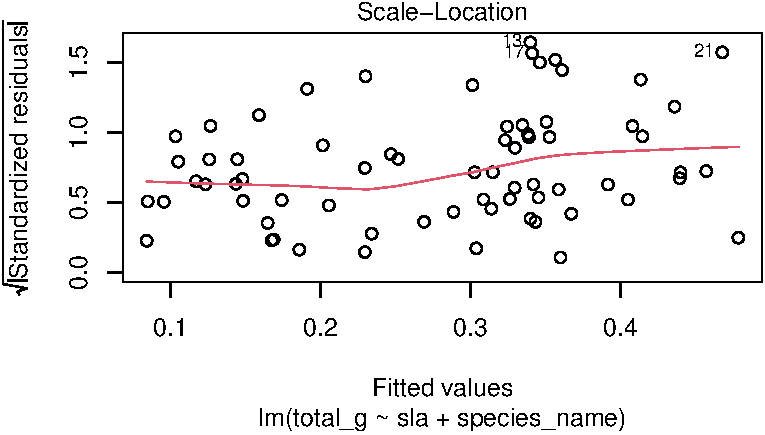
\includegraphics{Odile_Gabbiani_homework-03_files/figure-pdf/unnamed-chunk-10-3.pdf}

}

\end{figure}

\begin{figure}[H]

{\centering 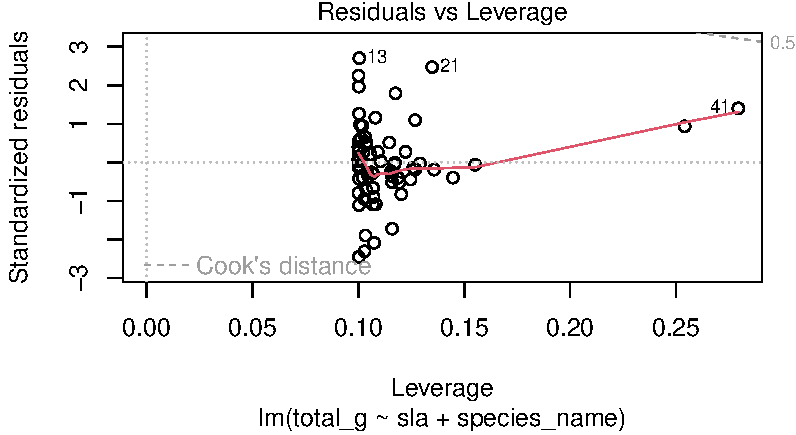
\includegraphics{Odile_Gabbiani_homework-03_files/figure-pdf/unnamed-chunk-10-4.pdf}

}

\end{figure}

\begin{Shaded}
\begin{Highlighting}[]
\NormalTok{model4 }\OtherTok{\textless{}{-}} \FunctionTok{lm}\NormalTok{(total\_g }\SpecialCharTok{\textasciitilde{}}\NormalTok{ water\_treatment }\SpecialCharTok{+}\NormalTok{ species\_name, }
             \AttributeTok{data =}\NormalTok{ drought\_exp\_clean)}
\FunctionTok{plot}\NormalTok{(model4)}
\end{Highlighting}
\end{Shaded}

\begin{figure}[H]

{\centering 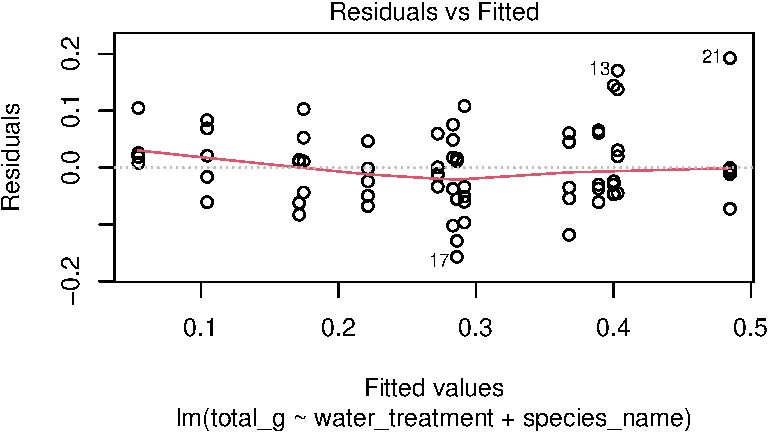
\includegraphics{Odile_Gabbiani_homework-03_files/figure-pdf/unnamed-chunk-11-1.pdf}

}

\end{figure}

\begin{figure}[H]

{\centering 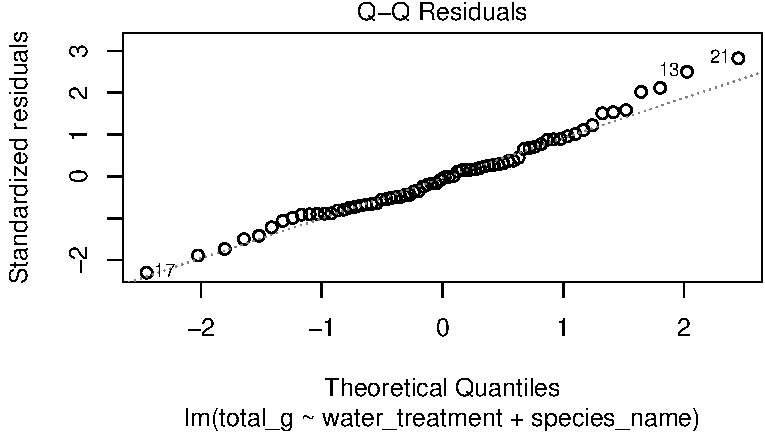
\includegraphics{Odile_Gabbiani_homework-03_files/figure-pdf/unnamed-chunk-11-2.pdf}

}

\end{figure}

\begin{figure}[H]

{\centering 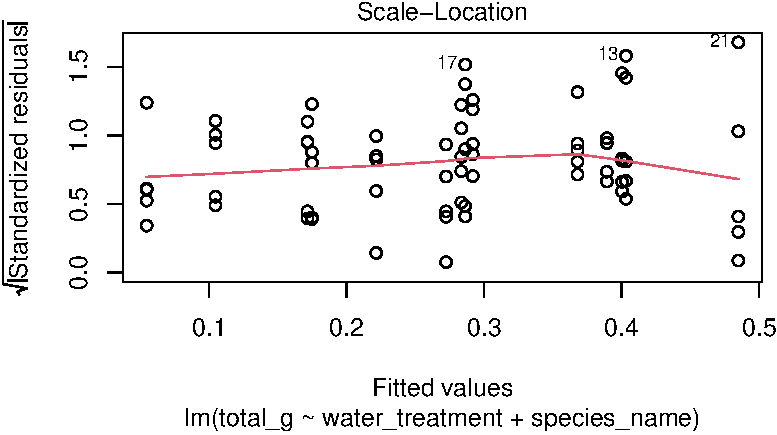
\includegraphics{Odile_Gabbiani_homework-03_files/figure-pdf/unnamed-chunk-11-3.pdf}

}

\end{figure}

\begin{figure}[H]

{\centering 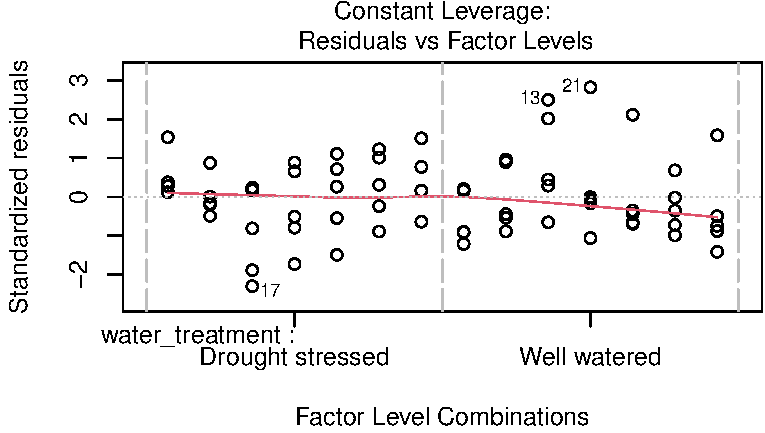
\includegraphics{Odile_Gabbiani_homework-03_files/figure-pdf/unnamed-chunk-11-4.pdf}

}

\end{figure}

\begin{Shaded}
\begin{Highlighting}[]
\NormalTok{model.sel }\OtherTok{\textless{}{-}} \FunctionTok{model.sel}\NormalTok{(model0,}
\NormalTok{          model1, }
\NormalTok{          model2, }
\NormalTok{          model3, }
\NormalTok{          model4)}

\NormalTok{flextable}\SpecialCharTok{::}\FunctionTok{as\_flextable}\NormalTok{(model.sel)}
\end{Highlighting}
\end{Shaded}

\global\setlength{\Oldarrayrulewidth}{\arrayrulewidth}

\global\setlength{\Oldtabcolsep}{\tabcolsep}

\setlength{\tabcolsep}{2pt}

\renewcommand*{\arraystretch}{1.5}



\providecommand{\ascline}[3]{\noalign{\global\arrayrulewidth #1}\arrayrulecolor[HTML]{#2}\cline{#3}}

\begin{longtable*}[c]{|p{0.98in}|p{0.83in}|p{1.27in}|p{1.39in}|p{0.75in}|p{0.83in}|p{0.83in}|p{0.83in}|p{1.26in}}



\ascline{1.5pt}{666666}{1-9}

\multicolumn{1}{>{\raggedleft}m{\dimexpr 0.98in+0\tabcolsep}}{\textcolor[HTML]{000000}{\fontsize{11}{11}\selectfont{(Intercept)}}} & \multicolumn{1}{>{\raggedleft}m{\dimexpr 0.83in+0\tabcolsep}}{\textcolor[HTML]{000000}{\fontsize{11}{11}\selectfont{sla}}} & \multicolumn{1}{>{\raggedright}m{\dimexpr 1.27in+0\tabcolsep}}{\textcolor[HTML]{000000}{\fontsize{11}{11}\selectfont{species\_name}}} & \multicolumn{1}{>{\raggedright}m{\dimexpr 1.39in+0\tabcolsep}}{\textcolor[HTML]{000000}{\fontsize{11}{11}\selectfont{water\_treatment}}} & \multicolumn{1}{>{\raggedleft}m{\dimexpr 0.75in+0\tabcolsep}}{\textcolor[HTML]{000000}{\fontsize{11}{11}\selectfont{df}}} & \multicolumn{1}{>{\raggedleft}m{\dimexpr 0.83in+0\tabcolsep}}{\textcolor[HTML]{000000}{\fontsize{11}{11}\selectfont{logLik}}} & \multicolumn{1}{>{\raggedleft}m{\dimexpr 0.83in+0\tabcolsep}}{\textcolor[HTML]{000000}{\fontsize{11}{11}\selectfont{AICc}}} & \multicolumn{1}{>{\raggedleft}m{\dimexpr 0.83in+0\tabcolsep}}{\textcolor[HTML]{000000}{\fontsize{11}{11}\selectfont{delta}}} & \multicolumn{1}{>{\raggedleft}m{\dimexpr 1.26in+0\tabcolsep}}{\textcolor[HTML]{000000}{\fontsize{11}{11}\selectfont{weight}}} \\





\multicolumn{1}{>{\raggedleft}m{\dimexpr 0.98in+0\tabcolsep}}{\textcolor[HTML]{999999}{\fontsize{11}{11}\selectfont{numeric}}} & \multicolumn{1}{>{\raggedleft}m{\dimexpr 0.83in+0\tabcolsep}}{\textcolor[HTML]{999999}{\fontsize{11}{11}\selectfont{numeric}}} & \multicolumn{1}{>{\raggedright}m{\dimexpr 1.27in+0\tabcolsep}}{\textcolor[HTML]{999999}{\fontsize{11}{11}\selectfont{factor}}} & \multicolumn{1}{>{\raggedright}m{\dimexpr 1.39in+0\tabcolsep}}{\textcolor[HTML]{999999}{\fontsize{11}{11}\selectfont{factor}}} & \multicolumn{1}{>{\raggedleft}m{\dimexpr 0.75in+0\tabcolsep}}{\textcolor[HTML]{999999}{\fontsize{11}{11}\selectfont{integer}}} & \multicolumn{1}{>{\raggedleft}m{\dimexpr 0.83in+0\tabcolsep}}{\textcolor[HTML]{999999}{\fontsize{11}{11}\selectfont{numeric}}} & \multicolumn{1}{>{\raggedleft}m{\dimexpr 0.83in+0\tabcolsep}}{\textcolor[HTML]{999999}{\fontsize{11}{11}\selectfont{numeric}}} & \multicolumn{1}{>{\raggedleft}m{\dimexpr 0.83in+0\tabcolsep}}{\textcolor[HTML]{999999}{\fontsize{11}{11}\selectfont{numeric}}} & \multicolumn{1}{>{\raggedleft}m{\dimexpr 1.26in+0\tabcolsep}}{\textcolor[HTML]{999999}{\fontsize{11}{11}\selectfont{model.weights}}} \\

\ascline{1.5pt}{666666}{1-9}\endfirsthead 

\ascline{1.5pt}{666666}{1-9}

\multicolumn{1}{>{\raggedleft}m{\dimexpr 0.98in+0\tabcolsep}}{\textcolor[HTML]{000000}{\fontsize{11}{11}\selectfont{(Intercept)}}} & \multicolumn{1}{>{\raggedleft}m{\dimexpr 0.83in+0\tabcolsep}}{\textcolor[HTML]{000000}{\fontsize{11}{11}\selectfont{sla}}} & \multicolumn{1}{>{\raggedright}m{\dimexpr 1.27in+0\tabcolsep}}{\textcolor[HTML]{000000}{\fontsize{11}{11}\selectfont{species\_name}}} & \multicolumn{1}{>{\raggedright}m{\dimexpr 1.39in+0\tabcolsep}}{\textcolor[HTML]{000000}{\fontsize{11}{11}\selectfont{water\_treatment}}} & \multicolumn{1}{>{\raggedleft}m{\dimexpr 0.75in+0\tabcolsep}}{\textcolor[HTML]{000000}{\fontsize{11}{11}\selectfont{df}}} & \multicolumn{1}{>{\raggedleft}m{\dimexpr 0.83in+0\tabcolsep}}{\textcolor[HTML]{000000}{\fontsize{11}{11}\selectfont{logLik}}} & \multicolumn{1}{>{\raggedleft}m{\dimexpr 0.83in+0\tabcolsep}}{\textcolor[HTML]{000000}{\fontsize{11}{11}\selectfont{AICc}}} & \multicolumn{1}{>{\raggedleft}m{\dimexpr 0.83in+0\tabcolsep}}{\textcolor[HTML]{000000}{\fontsize{11}{11}\selectfont{delta}}} & \multicolumn{1}{>{\raggedleft}m{\dimexpr 1.26in+0\tabcolsep}}{\textcolor[HTML]{000000}{\fontsize{11}{11}\selectfont{weight}}} \\





\multicolumn{1}{>{\raggedleft}m{\dimexpr 0.98in+0\tabcolsep}}{\textcolor[HTML]{999999}{\fontsize{11}{11}\selectfont{numeric}}} & \multicolumn{1}{>{\raggedleft}m{\dimexpr 0.83in+0\tabcolsep}}{\textcolor[HTML]{999999}{\fontsize{11}{11}\selectfont{numeric}}} & \multicolumn{1}{>{\raggedright}m{\dimexpr 1.27in+0\tabcolsep}}{\textcolor[HTML]{999999}{\fontsize{11}{11}\selectfont{factor}}} & \multicolumn{1}{>{\raggedright}m{\dimexpr 1.39in+0\tabcolsep}}{\textcolor[HTML]{999999}{\fontsize{11}{11}\selectfont{factor}}} & \multicolumn{1}{>{\raggedleft}m{\dimexpr 0.75in+0\tabcolsep}}{\textcolor[HTML]{999999}{\fontsize{11}{11}\selectfont{integer}}} & \multicolumn{1}{>{\raggedleft}m{\dimexpr 0.83in+0\tabcolsep}}{\textcolor[HTML]{999999}{\fontsize{11}{11}\selectfont{numeric}}} & \multicolumn{1}{>{\raggedleft}m{\dimexpr 0.83in+0\tabcolsep}}{\textcolor[HTML]{999999}{\fontsize{11}{11}\selectfont{numeric}}} & \multicolumn{1}{>{\raggedleft}m{\dimexpr 0.83in+0\tabcolsep}}{\textcolor[HTML]{999999}{\fontsize{11}{11}\selectfont{numeric}}} & \multicolumn{1}{>{\raggedleft}m{\dimexpr 1.26in+0\tabcolsep}}{\textcolor[HTML]{999999}{\fontsize{11}{11}\selectfont{model.weights}}} \\

\ascline{1.5pt}{666666}{1-9}\endhead



\multicolumn{1}{>{\raggedleft}m{\dimexpr 0.98in+0\tabcolsep}}{\textcolor[HTML]{000000}{\fontsize{11}{11}\selectfont{0.1}}} & \multicolumn{1}{>{\raggedleft}m{\dimexpr 0.83in+0\tabcolsep}}{\textcolor[HTML]{000000}{\fontsize{11}{11}\selectfont{}}} & \multicolumn{1}{>{\raggedright}m{\dimexpr 1.27in+0\tabcolsep}}{\textcolor[HTML]{000000}{\fontsize{11}{11}\selectfont{+}}} & \multicolumn{1}{>{\raggedright}m{\dimexpr 1.39in+0\tabcolsep}}{\textcolor[HTML]{000000}{\fontsize{11}{11}\selectfont{+}}} & \multicolumn{1}{>{\raggedleft}m{\dimexpr 0.75in+0\tabcolsep}}{\textcolor[HTML]{000000}{\fontsize{11}{11}\selectfont{9}}} & \multicolumn{1}{>{\raggedleft}m{\dimexpr 0.83in+0\tabcolsep}}{\textcolor[HTML]{000000}{\fontsize{11}{11}\selectfont{88.6}}} & \multicolumn{1}{>{\raggedleft}m{\dimexpr 0.83in+0\tabcolsep}}{\textcolor[HTML]{000000}{\fontsize{11}{11}\selectfont{-156.2}}} & \multicolumn{1}{>{\raggedleft}m{\dimexpr 0.83in+0\tabcolsep}}{\textcolor[HTML]{000000}{\fontsize{11}{11}\selectfont{0.0}}} & \multicolumn{1}{>{\raggedleft}m{\dimexpr 1.26in+0\tabcolsep}}{\textcolor[HTML]{000000}{\fontsize{11}{11}\selectfont{0.8}}} \\





\multicolumn{1}{>{\raggedleft}m{\dimexpr 0.98in+0\tabcolsep}}{\textcolor[HTML]{000000}{\fontsize{11}{11}\selectfont{0.1}}} & \multicolumn{1}{>{\raggedleft}m{\dimexpr 0.83in+0\tabcolsep}}{\textcolor[HTML]{000000}{\fontsize{11}{11}\selectfont{-0.0}}} & \multicolumn{1}{>{\raggedright}m{\dimexpr 1.27in+0\tabcolsep}}{\textcolor[HTML]{000000}{\fontsize{11}{11}\selectfont{+}}} & \multicolumn{1}{>{\raggedright}m{\dimexpr 1.39in+0\tabcolsep}}{\textcolor[HTML]{000000}{\fontsize{11}{11}\selectfont{+}}} & \multicolumn{1}{>{\raggedleft}m{\dimexpr 0.75in+0\tabcolsep}}{\textcolor[HTML]{000000}{\fontsize{11}{11}\selectfont{10}}} & \multicolumn{1}{>{\raggedleft}m{\dimexpr 0.83in+0\tabcolsep}}{\textcolor[HTML]{000000}{\fontsize{11}{11}\selectfont{88.7}}} & \multicolumn{1}{>{\raggedleft}m{\dimexpr 0.83in+0\tabcolsep}}{\textcolor[HTML]{000000}{\fontsize{11}{11}\selectfont{-153.8}}} & \multicolumn{1}{>{\raggedleft}m{\dimexpr 0.83in+0\tabcolsep}}{\textcolor[HTML]{000000}{\fontsize{11}{11}\selectfont{2.4}}} & \multicolumn{1}{>{\raggedleft}m{\dimexpr 1.26in+0\tabcolsep}}{\textcolor[HTML]{000000}{\fontsize{11}{11}\selectfont{0.2}}} \\





\multicolumn{1}{>{\raggedleft}m{\dimexpr 0.98in+0\tabcolsep}}{\textcolor[HTML]{000000}{\fontsize{11}{11}\selectfont{-0.0}}} & \multicolumn{1}{>{\raggedleft}m{\dimexpr 0.83in+0\tabcolsep}}{\textcolor[HTML]{000000}{\fontsize{11}{11}\selectfont{0.0}}} & \multicolumn{1}{>{\raggedright}m{\dimexpr 1.27in+0\tabcolsep}}{\textcolor[HTML]{000000}{\fontsize{11}{11}\selectfont{+}}} & \multicolumn{1}{>{\raggedright}m{\dimexpr 1.39in+0\tabcolsep}}{\textcolor[HTML]{000000}{\fontsize{11}{11}\selectfont{}}} & \multicolumn{1}{>{\raggedleft}m{\dimexpr 0.75in+0\tabcolsep}}{\textcolor[HTML]{000000}{\fontsize{11}{11}\selectfont{9}}} & \multicolumn{1}{>{\raggedleft}m{\dimexpr 0.83in+0\tabcolsep}}{\textcolor[HTML]{000000}{\fontsize{11}{11}\selectfont{72.5}}} & \multicolumn{1}{>{\raggedleft}m{\dimexpr 0.83in+0\tabcolsep}}{\textcolor[HTML]{000000}{\fontsize{11}{11}\selectfont{-124.1}}} & \multicolumn{1}{>{\raggedleft}m{\dimexpr 0.83in+0\tabcolsep}}{\textcolor[HTML]{000000}{\fontsize{11}{11}\selectfont{32.1}}} & \multicolumn{1}{>{\raggedleft}m{\dimexpr 1.26in+0\tabcolsep}}{\textcolor[HTML]{000000}{\fontsize{11}{11}\selectfont{0.0}}} \\





\multicolumn{1}{>{\raggedleft}m{\dimexpr 0.98in+0\tabcolsep}}{\textcolor[HTML]{000000}{\fontsize{11}{11}\selectfont{0.0}}} & \multicolumn{1}{>{\raggedleft}m{\dimexpr 0.83in+0\tabcolsep}}{\textcolor[HTML]{000000}{\fontsize{11}{11}\selectfont{0.0}}} & \multicolumn{1}{>{\raggedright}m{\dimexpr 1.27in+0\tabcolsep}}{\textcolor[HTML]{000000}{\fontsize{11}{11}\selectfont{}}} & \multicolumn{1}{>{\raggedright}m{\dimexpr 1.39in+0\tabcolsep}}{\textcolor[HTML]{000000}{\fontsize{11}{11}\selectfont{+}}} & \multicolumn{1}{>{\raggedleft}m{\dimexpr 0.75in+0\tabcolsep}}{\textcolor[HTML]{000000}{\fontsize{11}{11}\selectfont{4}}} & \multicolumn{1}{>{\raggedleft}m{\dimexpr 0.83in+0\tabcolsep}}{\textcolor[HTML]{000000}{\fontsize{11}{11}\selectfont{52.2}}} & \multicolumn{1}{>{\raggedleft}m{\dimexpr 0.83in+0\tabcolsep}}{\textcolor[HTML]{000000}{\fontsize{11}{11}\selectfont{-95.8}}} & \multicolumn{1}{>{\raggedleft}m{\dimexpr 0.83in+0\tabcolsep}}{\textcolor[HTML]{000000}{\fontsize{11}{11}\selectfont{60.4}}} & \multicolumn{1}{>{\raggedleft}m{\dimexpr 1.26in+0\tabcolsep}}{\textcolor[HTML]{000000}{\fontsize{11}{11}\selectfont{0.0}}} \\





\multicolumn{1}{>{\raggedleft}m{\dimexpr 0.98in+0\tabcolsep}}{\textcolor[HTML]{000000}{\fontsize{11}{11}\selectfont{0.3}}} & \multicolumn{1}{>{\raggedleft}m{\dimexpr 0.83in+0\tabcolsep}}{\textcolor[HTML]{000000}{\fontsize{11}{11}\selectfont{}}} & \multicolumn{1}{>{\raggedright}m{\dimexpr 1.27in+0\tabcolsep}}{\textcolor[HTML]{000000}{\fontsize{11}{11}\selectfont{}}} & \multicolumn{1}{>{\raggedright}m{\dimexpr 1.39in+0\tabcolsep}}{\textcolor[HTML]{000000}{\fontsize{11}{11}\selectfont{}}} & \multicolumn{1}{>{\raggedleft}m{\dimexpr 0.75in+0\tabcolsep}}{\textcolor[HTML]{000000}{\fontsize{11}{11}\selectfont{2}}} & \multicolumn{1}{>{\raggedleft}m{\dimexpr 0.83in+0\tabcolsep}}{\textcolor[HTML]{000000}{\fontsize{11}{11}\selectfont{39.6}}} & \multicolumn{1}{>{\raggedleft}m{\dimexpr 0.83in+0\tabcolsep}}{\textcolor[HTML]{000000}{\fontsize{11}{11}\selectfont{-75.0}}} & \multicolumn{1}{>{\raggedleft}m{\dimexpr 0.83in+0\tabcolsep}}{\textcolor[HTML]{000000}{\fontsize{11}{11}\selectfont{81.2}}} & \multicolumn{1}{>{\raggedleft}m{\dimexpr 1.26in+0\tabcolsep}}{\textcolor[HTML]{000000}{\fontsize{11}{11}\selectfont{0.0}}} \\

\ascline{1.5pt}{666666}{1-9}



\multicolumn{9}{>{\raggedright}m{\dimexpr 8.97in+16\tabcolsep}}{\textcolor[HTML]{000000}{\fontsize{11}{11}\selectfont{n:\ 5}}} \\

\ascline{1.5pt}{666666}{1-9}



\end{longtable*}



\arrayrulecolor[HTML]{000000}

\global\setlength{\arrayrulewidth}{\Oldarrayrulewidth}

\global\setlength{\tabcolsep}{\Oldtabcolsep}

\renewcommand*{\arraystretch}{1}

\begin{Shaded}
\begin{Highlighting}[]
\NormalTok{modelsummary}\SpecialCharTok{::}\FunctionTok{modelsummary}\NormalTok{( }\CommentTok{\# this function takes a list of models}
  \FunctionTok{list}\NormalTok{( }
    \StringTok{"null"} \OtherTok{=}\NormalTok{ model0, }\CommentTok{\# "model name" = model object}
    \StringTok{"model 1"} \OtherTok{=}\NormalTok{ model1,}
    \StringTok{"model 2"} \OtherTok{=}\NormalTok{ model2,}
    \StringTok{"model 3"} \OtherTok{=}\NormalTok{ model3, }
    \StringTok{"model 4"} \OtherTok{=}\NormalTok{ model4), }
  \AttributeTok{title =} \StringTok{"Table 1: Model Comparison"}\NormalTok{, }
  \AttributeTok{gof\_map =} \FunctionTok{c}\NormalTok{(}\StringTok{"aic"}\NormalTok{)}
\NormalTok{) }
\end{Highlighting}
\end{Shaded}

\begin{table}
\centering
\begin{talltblr}[         %% tabularray outer open
caption={Table 1: Model Comparison},
]                     %% tabularray outer close
{                     %% tabularray inner open
colspec={Q[]Q[]Q[]Q[]Q[]Q[]},
column{1}={halign=l,},
column{2}={halign=c,},
column{3}={halign=c,},
column{4}={halign=c,},
column{5}={halign=c,},
column{6}={halign=c,},
hline{20}={1,2,3,4,5,6}{solid, 0.05em, black},
}                     %% tabularray inner close
\toprule
& null & model 1 & model 2 & model 3 & model 4 \\ \midrule %% TinyTableHeader
(Intercept)                              & \num{0.279}   & \num{0.080}   & \num{0.047}   & \num{-0.033}  & \num{0.055}   \\
& (\num{0.017}) & (\num{0.056}) & (\num{0.054}) & (\num{0.067}) & (\num{0.025}) \\
sla                                      &                & \num{0.000}   & \num{0.001}   & \num{0.001}   &                \\
&                & (\num{0.000}) & (\num{0.000}) & (\num{0.001}) &                \\
water\_treatmentWell watered            &                & \num{0.122}   & \num{0.090}   &                & \num{0.117}   \\
&                & (\num{0.020}) & (\num{0.029}) &                & (\num{0.017}) \\
species\_nameEncelia californica        &                & \num{0.238}   &                & \num{0.115}   & \num{0.218}   \\
&                & (\num{0.051}) &                & (\num{0.059}) & (\num{0.032}) \\
species\_nameEschscholzia californica   &                & \num{0.234}   &                & \num{0.222}   & \num{0.232}   \\
&                & (\num{0.033}) &                & (\num{0.041}) & (\num{0.032}) \\
species\_nameGrindelia camporum         &                & \num{0.330}   &                & \num{0.226}   & \num{0.313}   \\
&                & (\num{0.047}) &                & (\num{0.054}) & (\num{0.032}) \\
species\_nameNasella pulchra            &                & \num{0.241}   &                & \num{0.168}   & \num{0.229}   \\
&                & (\num{0.040}) &                & (\num{0.048}) & (\num{0.032}) \\
species\_namePenstemon centranthifolius &                & \num{0.061}   &                & \num{-0.006}  & \num{0.050}   \\
&                & (\num{0.039}) &                & (\num{0.047}) & (\num{0.032}) \\
species\_nameSalvia leucophylla         &                & \num{0.117}   &                & \num{0.139}   & \num{0.120}   \\
&                & (\num{0.033}) &                & (\num{0.041}) & (\num{0.032}) \\
AIC                                      & \num{-75.2}   & \num{-157.5}  & \num{-96.4}   & \num{-127.1}  & \num{-159.2}  \\
\bottomrule
\end{talltblr}
\end{table}

\begin{Shaded}
\begin{Highlighting}[]
\NormalTok{model\_preds }\OtherTok{\textless{}{-}} \FunctionTok{ggpredict}\NormalTok{(model4, }
                         \AttributeTok{terms =} \FunctionTok{c}\NormalTok{(}\StringTok{"water\_treatment"}\NormalTok{, }
                                   \StringTok{"species\_name"}\NormalTok{))}
\end{Highlighting}
\end{Shaded}

\begin{Shaded}
\begin{Highlighting}[]
\FunctionTok{plot}\NormalTok{(model\_preds, }\CommentTok{\# model predictions}
     \AttributeTok{limit\_range =} \ConstantTok{TRUE}\NormalTok{, }\CommentTok{\# limit the range of predictions to the range of predictor values}
     \AttributeTok{show\_data =} \ConstantTok{TRUE}\NormalTok{) }\SpecialCharTok{+} \CommentTok{\# show the underlying data}
  \CommentTok{\# everything below this is ggplot() stuff}
  \FunctionTok{theme\_classic}\NormalTok{() }\SpecialCharTok{+} \CommentTok{\# classic theme}
  \FunctionTok{labs}\NormalTok{(}\AttributeTok{title =} \StringTok{"Preliminary model visualization"}\NormalTok{) }\SpecialCharTok{+} \CommentTok{\# plot title}
  \FunctionTok{theme}\NormalTok{(}\AttributeTok{panel.grid =} \FunctionTok{element\_blank}\NormalTok{()) }\CommentTok{\# getting rid of gridlines}
\end{Highlighting}
\end{Shaded}

\begin{figure}[H]

{\centering 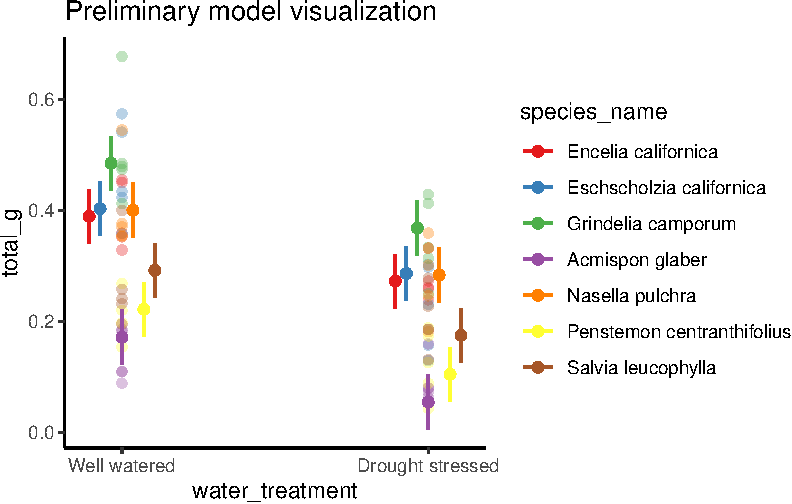
\includegraphics{Odile_Gabbiani_homework-03_files/figure-pdf/unnamed-chunk-15-1.pdf}

}

\end{figure}

\begin{Shaded}
\begin{Highlighting}[]
\NormalTok{model\_preds\_for\_plotting }\OtherTok{\textless{}{-}}\NormalTok{ model\_preds }\SpecialCharTok{\%\textgreater{}\%} 
  \FunctionTok{rename}\NormalTok{(}\AttributeTok{water\_treatment =}\NormalTok{ x,}
         \AttributeTok{species\_name =}\NormalTok{ group)}

\CommentTok{\# use View(model\_preds\_for\_plotting) }
\CommentTok{\# to compare this to the original model\_preds data frame}

\FunctionTok{ggplot}\NormalTok{() }\SpecialCharTok{+}
  \CommentTok{\# underlying data}
  \FunctionTok{geom\_point}\NormalTok{(}\AttributeTok{data =}\NormalTok{ drought\_exp\_clean,}
             \AttributeTok{alpha =} \FloatTok{0.3}\NormalTok{,}
             \FunctionTok{aes}\NormalTok{(}\AttributeTok{x =}\NormalTok{ water\_treatment,}
                 \AttributeTok{y =}\NormalTok{ total\_g,}
                 \AttributeTok{color =}\NormalTok{ water\_treatment)) }\SpecialCharTok{+}
  \CommentTok{\# model prediction 95\% CI ribbon}
\FunctionTok{geom\_errorbar}\NormalTok{(}\AttributeTok{data =}\NormalTok{ model\_preds\_for\_plotting,}
             \FunctionTok{aes}\NormalTok{(}\AttributeTok{x =}\NormalTok{ water\_treatment, }
                  \AttributeTok{y =}\NormalTok{ predicted,}
                  \AttributeTok{ymin =}\NormalTok{ conf.low,}
                  \AttributeTok{ymax =}\NormalTok{ conf.high,}
                  \AttributeTok{fill =}\NormalTok{ water\_treatment),}
              \AttributeTok{alpha =} \FloatTok{0.2}\NormalTok{, }\AttributeTok{width =} \FloatTok{0.2}\NormalTok{) }\SpecialCharTok{+}
  \CommentTok{\# model prediction lines}
  \FunctionTok{geom\_point}\NormalTok{(}\AttributeTok{data =}\NormalTok{ model\_preds\_for\_plotting,}
            \FunctionTok{aes}\NormalTok{(}\AttributeTok{x =}\NormalTok{ water\_treatment, }
                \AttributeTok{y =}\NormalTok{ predicted,}
                \AttributeTok{color =}\NormalTok{ water\_treatment)) }\SpecialCharTok{+}
  \CommentTok{\# cleaner theme}
  \FunctionTok{theme\_classic}\NormalTok{() }\SpecialCharTok{+}
  \CommentTok{\# creating different panels for species}
  \FunctionTok{facet\_wrap}\NormalTok{(}\SpecialCharTok{\textasciitilde{}}\NormalTok{species\_name) }\SpecialCharTok{+} 
  \FunctionTok{theme}\NormalTok{(}\AttributeTok{legend.position =} \StringTok{"none"}\NormalTok{) }\SpecialCharTok{+} 
  \FunctionTok{labs}\NormalTok{(}\AttributeTok{x =} \StringTok{"Water Treatment"}\NormalTok{, }
       \AttributeTok{y =} \StringTok{"Total Biomass (g)"}\NormalTok{, }
       \AttributeTok{title =} \StringTok{"Figure 1: Total Biomass (g) as predicted by Water Treatment and Plant Species"}\NormalTok{) }\SpecialCharTok{+} 
  \FunctionTok{scale\_color\_manual}\NormalTok{(}\AttributeTok{values =} \FunctionTok{c}\NormalTok{(}\StringTok{"Well watered"} \OtherTok{=} \StringTok{"orchid3"}\NormalTok{, }
                                \StringTok{"Drought stressed"} \OtherTok{=} \StringTok{"olivedrab4"}\NormalTok{))}
\end{Highlighting}
\end{Shaded}

\begin{figure}[H]

{\centering 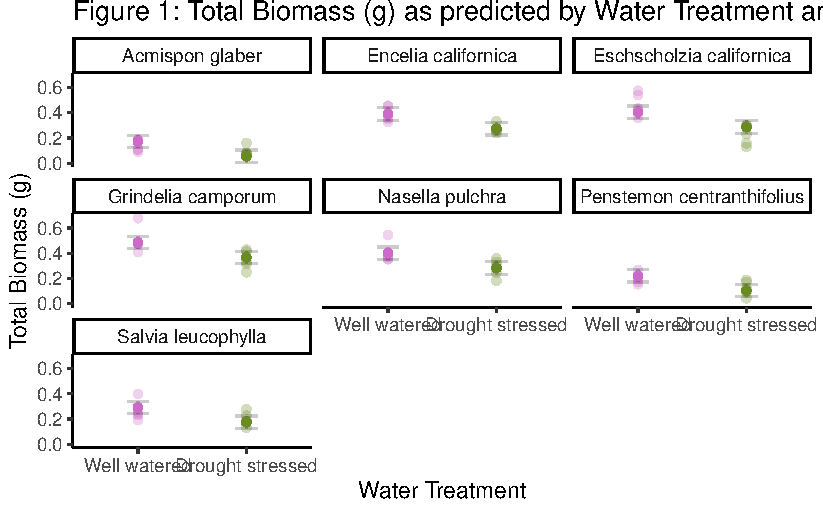
\includegraphics{Odile_Gabbiani_homework-03_files/figure-pdf/unnamed-chunk-16-1.pdf}

}

\end{figure}

\begin{enumerate}
\def\labelenumi{\arabic{enumi}.}
\setcounter{enumi}{1}
\tightlist
\item
  Affective Visualization
\end{enumerate}

\begin{enumerate}
\def\labelenumi{\alph{enumi}.}
\item
  The data I took over the course of this class describes the number and
  species of birds seen perching on an artificial floating wetland
  island (FWI) on the UCSB Lagoon. An affectively visualization of my
  data could consist of birds sitting on pilings of different heights to
  represent how often each bird species was seen. Each piling would
  correspond to a different bird and that would be represented by having
  that specific species sitting atop it. While the pilings don't
  represent exactly where the birds were seen perching, they do give an
  idea of how many birds of each species were seen.
\item
\item
\item
  UCSB Lagoon Birds: this piece shows the number of bird species seen
  perching on an artificial floating wetland island (FWI) at the UCSB
  Lagoon over a period of five months, from January to May 2024. Each
  piling represents a different observed bird species and the piling's
  heights represent how many of those birds were seen. This piece is a
  Caran D'ache color pencil drawing that also incorporates Archival Ink
  pens to outline certain aspects of the visualization. To make this, I
  first made a sketch of what I wanted it to look like, which I
  transferred onto paper. I found images of the six bird species seen on
  the UCSB Lagoon and I drew them on top of the pilings. I did
  everything in pencil first, then added color, and finished by adding
  touches of ink.
\end{enumerate}

\begin{enumerate}
\def\labelenumi{\arabic{enumi}.}
\setcounter{enumi}{2}
\tightlist
\item
  Statistical Critique
\end{enumerate}

\begin{enumerate}
\def\labelenumi{\alph{enumi}.}
\item
  To address their main research question (are CFWs effective in
  removing N and P from aquatic systems?), the authors used a variety of
  tests including Levene's Test, Kruskall Wallis Test, Spearman's R
  Correlation Coefficient, and Linear Regression. The authors did not
  include a visualization of their data in the article but they do have
  tables listing data points and showing the relationship between
  different variables. This is the table they included for the
  Spearman's R Correlation Coefficient.
\item
  To visualize their data, I would suggest the authors use
\end{enumerate}



\end{document}
